%%%%%%%%%%%%%%%%%%%%%%%%%%%%%%%%%%%%%%%%%
% Jacobs Landscape Poster
% LaTeX Template
% Version 1.0 (29/03/13)
%
% Created by:
% Computational Physics and Biophysics Group, Jacobs University
% https://teamwork.jacobs-university.de:8443/confluence/display/CoPandBiG/LaTeX+Poster
% 
% Further modified by:
% Nathaniel Johnston (nathaniel@njohnston.ca)
%
% This template has been downloaded from:
% http://www.LaTeXTemplates.com
%
% License:
% CC BY-NC-SA 3.0 (http://creativecommons.org/licenses/by-nc-sa/3.0/)
%
%%%%%%%%%%%%%%%%%%%%%%%%%%%%%%%%%%%%%%%%%

%----------------------------------------------------------------------------------------
%	PACKAGES AND OTHER DOCUMENT CONFIGURATIONS
%----------------------------------------------------------------------------------------

\documentclass[final]{beamer}

\usepackage[scale=1.24]{beamerposter} % Use the beamerposter package for laying out the poster
\definecolor{jhudarkblue}{RGB}{0, 45, 114}
\definecolor{jhulightblue}{cmyk}{56, 18, 0, 0}
\usetheme{confposter} % Use the confposter theme supplied with this template

\setbeamercolor{block title}{fg=jhulightblue,bg=white} % Colors of the block titles
\setbeamercolor{block body}{fg=black,bg=white} % Colors of the body of blocks
\setbeamercolor{block alerted title}{fg=white,bg=jhudarkblue} % Colors of the highlighted block titles
\setbeamercolor{block alerted body}{fg=black,bg=dblue!10} % Colors of the body of highlighted blocks
% Many more colors are available for use in beamerthemeconfposter.sty

%-----------------------------------------------------------
% Define the column widths and overall poster size
% To set effective sepwid, onecolwid and twocolwid values, first choose how many columns you want and how much separation you want between columns
% In this template, the separation width chosen is 0.024 of the paper width and a 4-column layout
% onecolwid should therefore be (1-(# of columns+1)*sepwid)/# of columns e.g. (1-(4+1)*0.024)/4 = 0.22
% Set twocolwid to be (2*onecolwid)+sepwid = 0.464
% Set threecolwid to be (3*onecolwid)+2*sepwid = 0.708

\newlength{\sepwid}
\newlength{\onecolwid}
\newlength{\twocolwid}
\newlength{\threecolwid}
\setlength{\paperwidth}{48in} % A0 width: 46.8in
\setlength{\paperheight}{36in} % A0 height: 33.1in
\setlength{\sepwid}{0.024\paperwidth} % Separation width (white space) between columns
\setlength{\onecolwid}{0.22\paperwidth} % Width of one column
\setlength{\twocolwid}{0.464\paperwidth} % Width of two columns
\setlength{\threecolwid}{0.708\paperwidth} % Width of three columns
\setlength{\topmargin}{-0.5in} % Reduce the top margin size
%-----------------------------------------------------------

\usepackage{graphicx}  % Required for including images
\usepackage{tikz}
\usepackage{booktabs} % Top and bottom rules for tables
\usepackage{svg}
%----------------------------------------------------------------------------------------
%	TITLE SECTION 
%----------------------------------------------------------------------------------------

\title{Off-shell Higgs boson Production Measurements} % Poster title

\author{Mohit Srivastav} % Author(s)

\institute{Johns Hopkins University, CMS Joint 4-Lepton Study Team (CJLST)} % Institution(s)

%----------------------------------------------------------------------------------------
% % below title
\addtobeamertemplate{headline}{}
{\begin{tikzpicture}[remember picture, overlay]
     %\node [anchor=north east, inner sep=3cm]  at (current page.north east)
     \node [shift={(-6.5cm, -9cm)}] at (current page.north east)
     {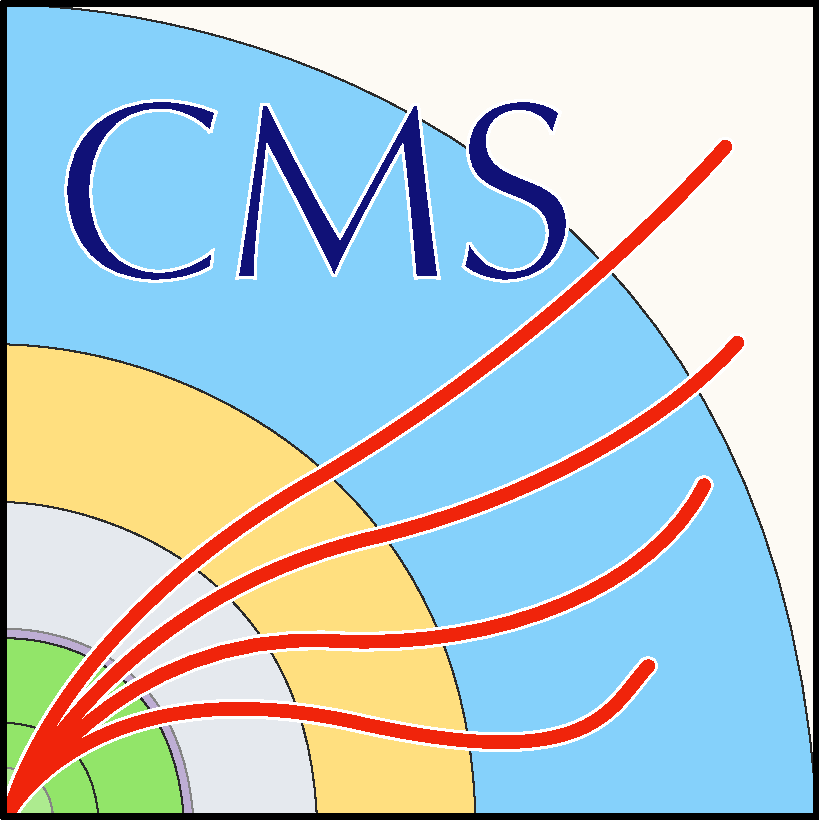
\includegraphics[height=10cm]{images/CMS_logo.pdf}};
  \end{tikzpicture}
  \begin{tikzpicture}[remember picture, overlay]
%      %\node [anchor=north east, inner sep=3cm]  at (current page.north east)
     \node [shift={(+6.5 cm, -9cm)}] at (current page.north west)
     {
\includegraphics[height=10cm]{images/JHU_seal.pdf}};
  \end{tikzpicture}
}
% %end

\begin{document}

\addtobeamertemplate{block end}{}{\vspace*{2ex}} % White space under blocks
\addtobeamertemplate{block alerted end}{}{\vspace*{2ex}} % White space under highlighted (alert) blocks

\setlength{\belowcaptionskip}{2ex} % White space under figures
\setlength\belowdisplayshortskip{2ex} % White space under equations

\begin{frame}[t] % The whole poster is enclosed in one beamer frame

\begin{columns}[t] % The whole poster consists of three major columns, the second of which is split into two columns twice - the [t] option aligns each column's content to the top

\begin{column}{\sepwid}\end{column} % Empty spacer column

\begin{column}{\onecolwid} % The first column

%----------------------------------------------------------------------------------------
%	OBJECTIVES
%----------------------------------------------------------------------------------------

\begin{alertblock}{Objectives}

Multiple measurements of off-shell Higgs boson production are presented:
\begin{enumerate}
\item The first test of Higgs substructure on CMS
\item The first measurement of $\kappa_\lambda$ in the off-shell region
\item The most precise indirect measurement of light-Yukawa couplings to date
\item Measurements of BSM phenomena in the EFT limit in gluon-fusion production
\item Constraints on the width with both heavy and light terms floated
\item A combination of all the Run-2 off-shell width measurements to date
\end{enumerate}


\end{alertblock}

%----------------------------------------------------------------------------------------
%	INTRODUCTION
%----------------------------------------------------------------------------------------

\begin{block}{The Off-shell Higgs boson}

The off-shell region of the Higgs boson is present in VV decays above $2m_V$,
and is characterized by a strong interference component with background.
The hallmark of the off-shell region is the independence from the the width,
as ~4 MeV $<<$ $2m_V$.
\begin{equation}
  \frac{\sigma(i \to H \to f)}{ds} \propto \frac{1}{(s-M_H^2)^2 + M_H^2\Gamma_H^2}
  \label{eq:width}
\end{equation}
\end{block}

%------------------------------------------------

% \begin{figure}
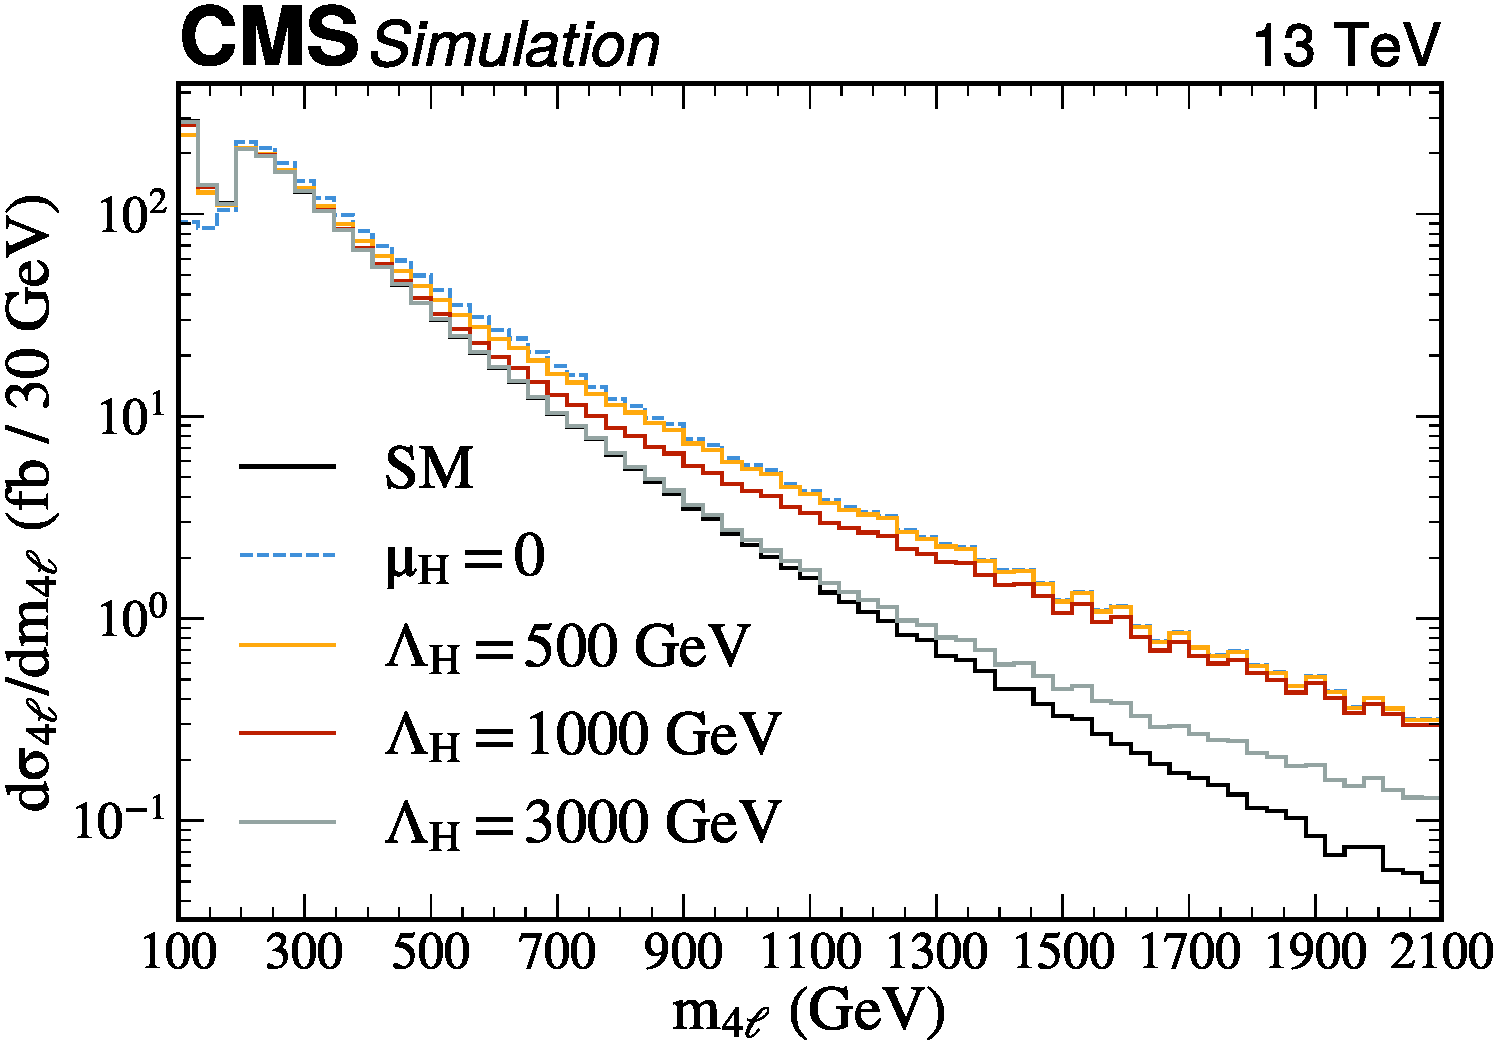
\includegraphics[width=\linewidth]{images/Struct_BSI.pdf}
% \caption{The EW evolution of the overall $4\ell$ distribution with varying Higgs signal strengths}
\label{fig:structure}
% \end{figure}

%----------------------------------------------------------------------------------------

\end{column} % End of the first column

\begin{column}{\sepwid}\end{column} % Empty spacer column

\begin{column}{\twocolwid} % Begin a column which is two columns wide (column 2)

\begin{columns}[t,totalwidth=\twocolwid] % Split up the two columns wide column

\begin{column}{\onecolwid}\vspace{-.6in} % The first column within column 2 (column 2.1)

%----------------------------------------------------------------------------------------
%	MATERIALS
%----------------------------------------------------------------------------------------

\begin{block}{Observables}
Observables crafted using MELA and MiLoMerge.
\begin{center}  
  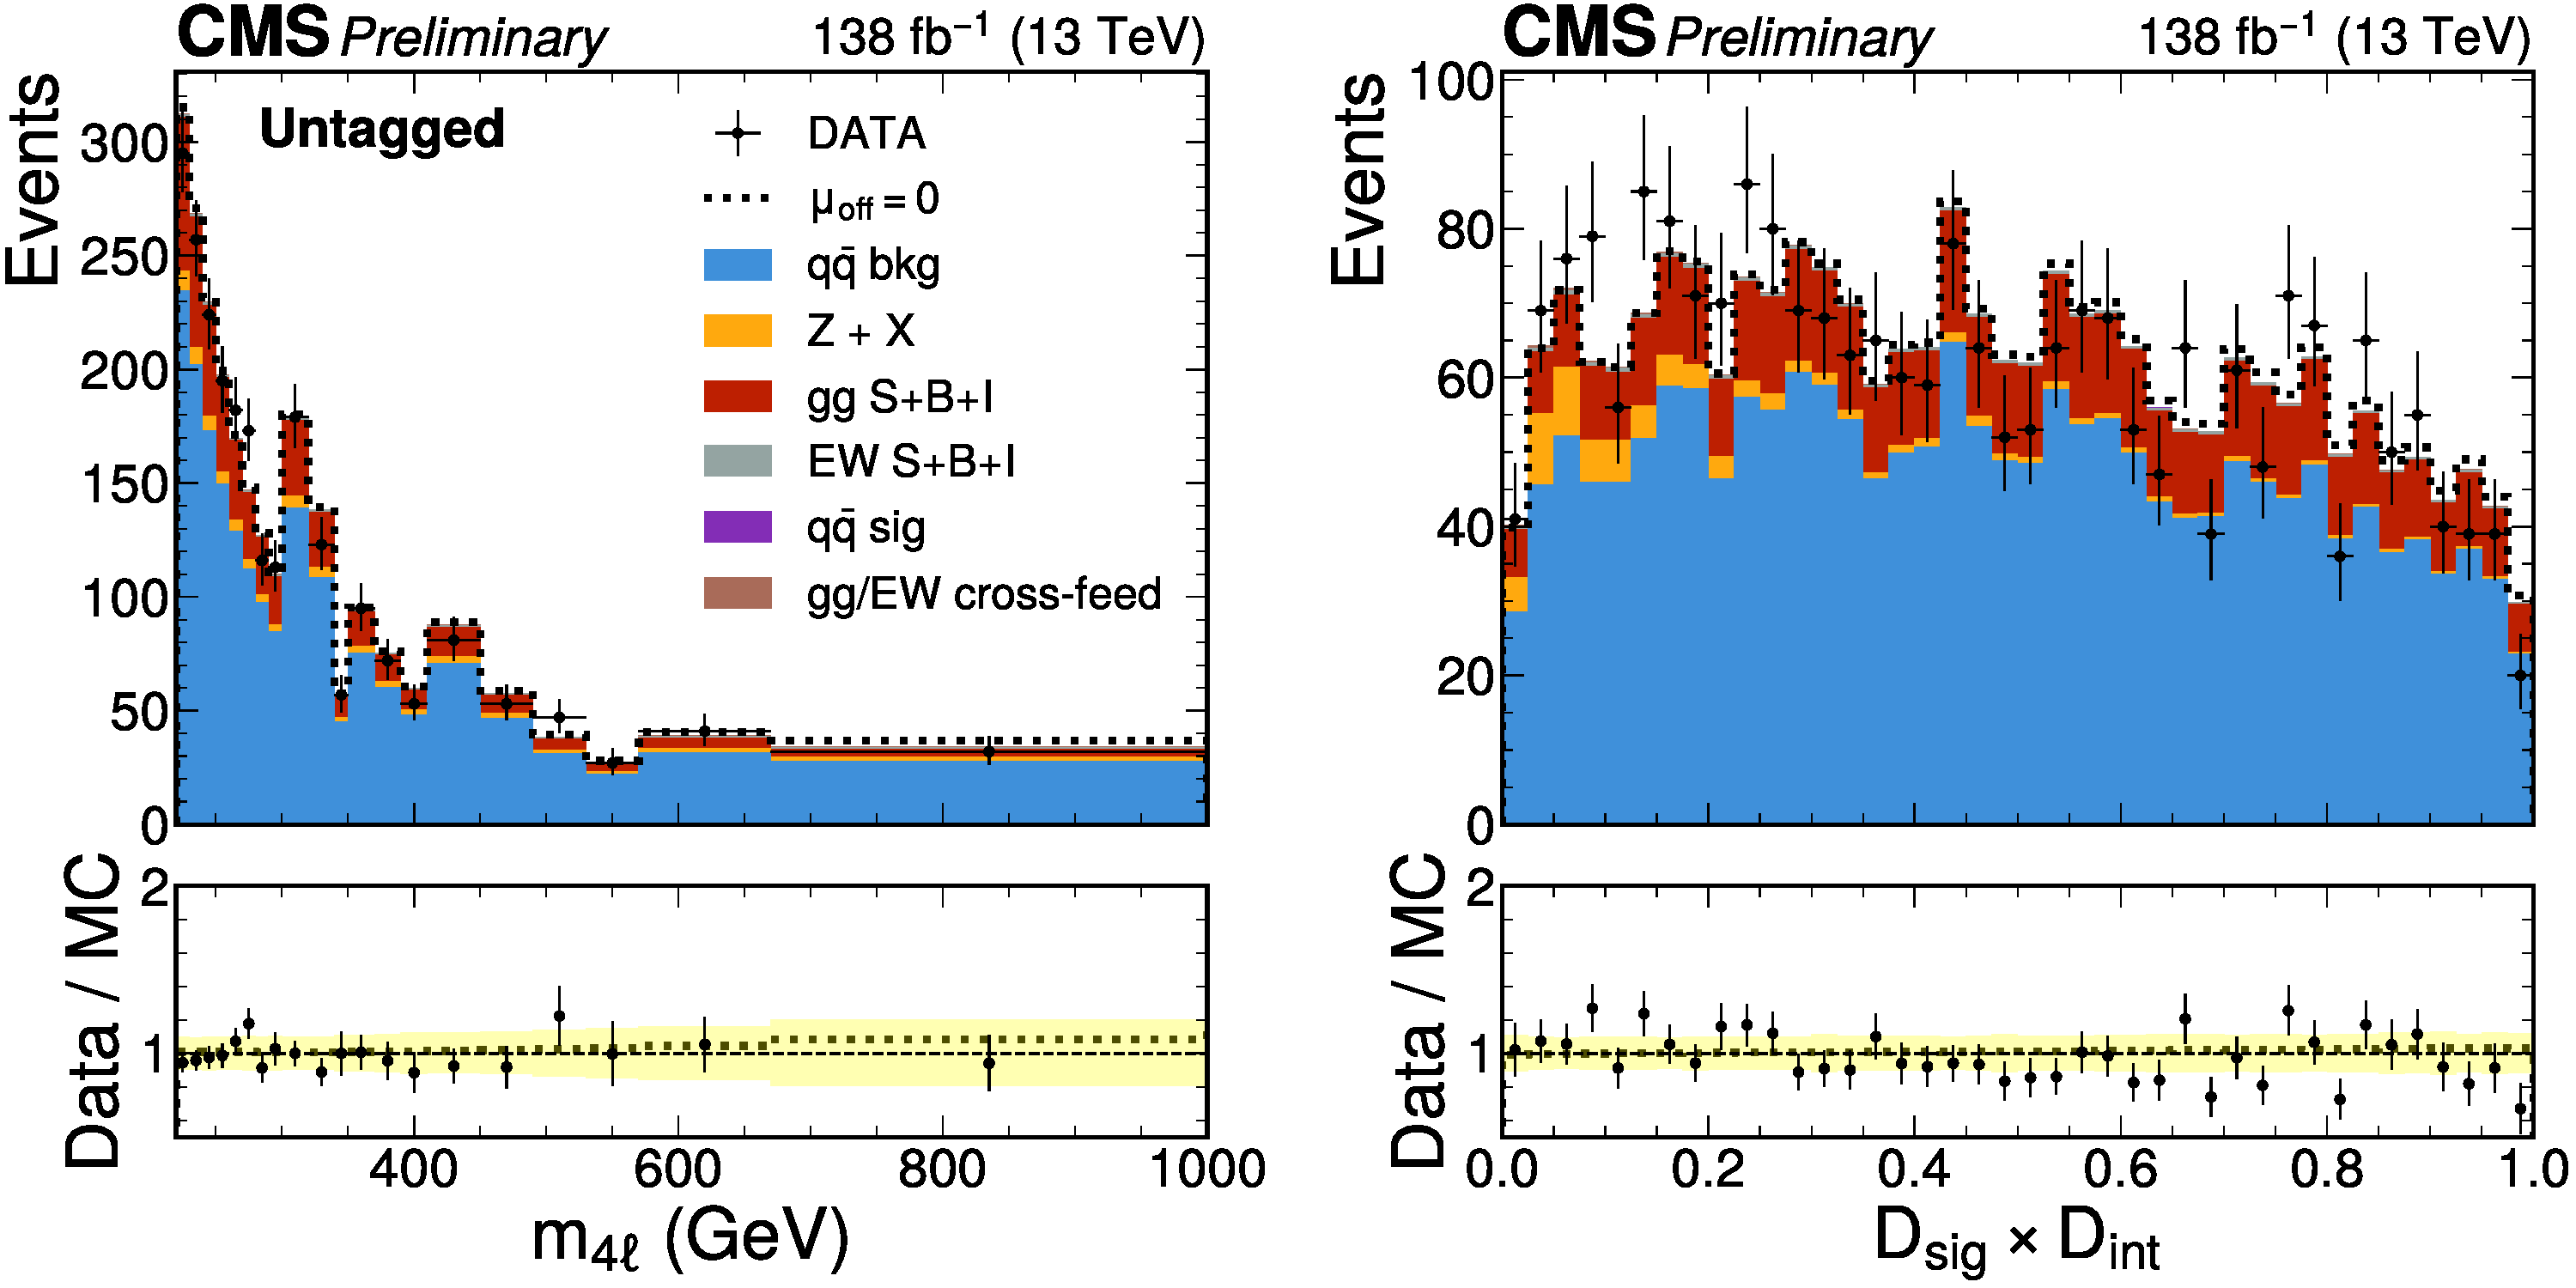
\includegraphics[trim={0 0 25cm 0},clip,  width=0.55\linewidth]{images/ratio_0.pdf}\\
  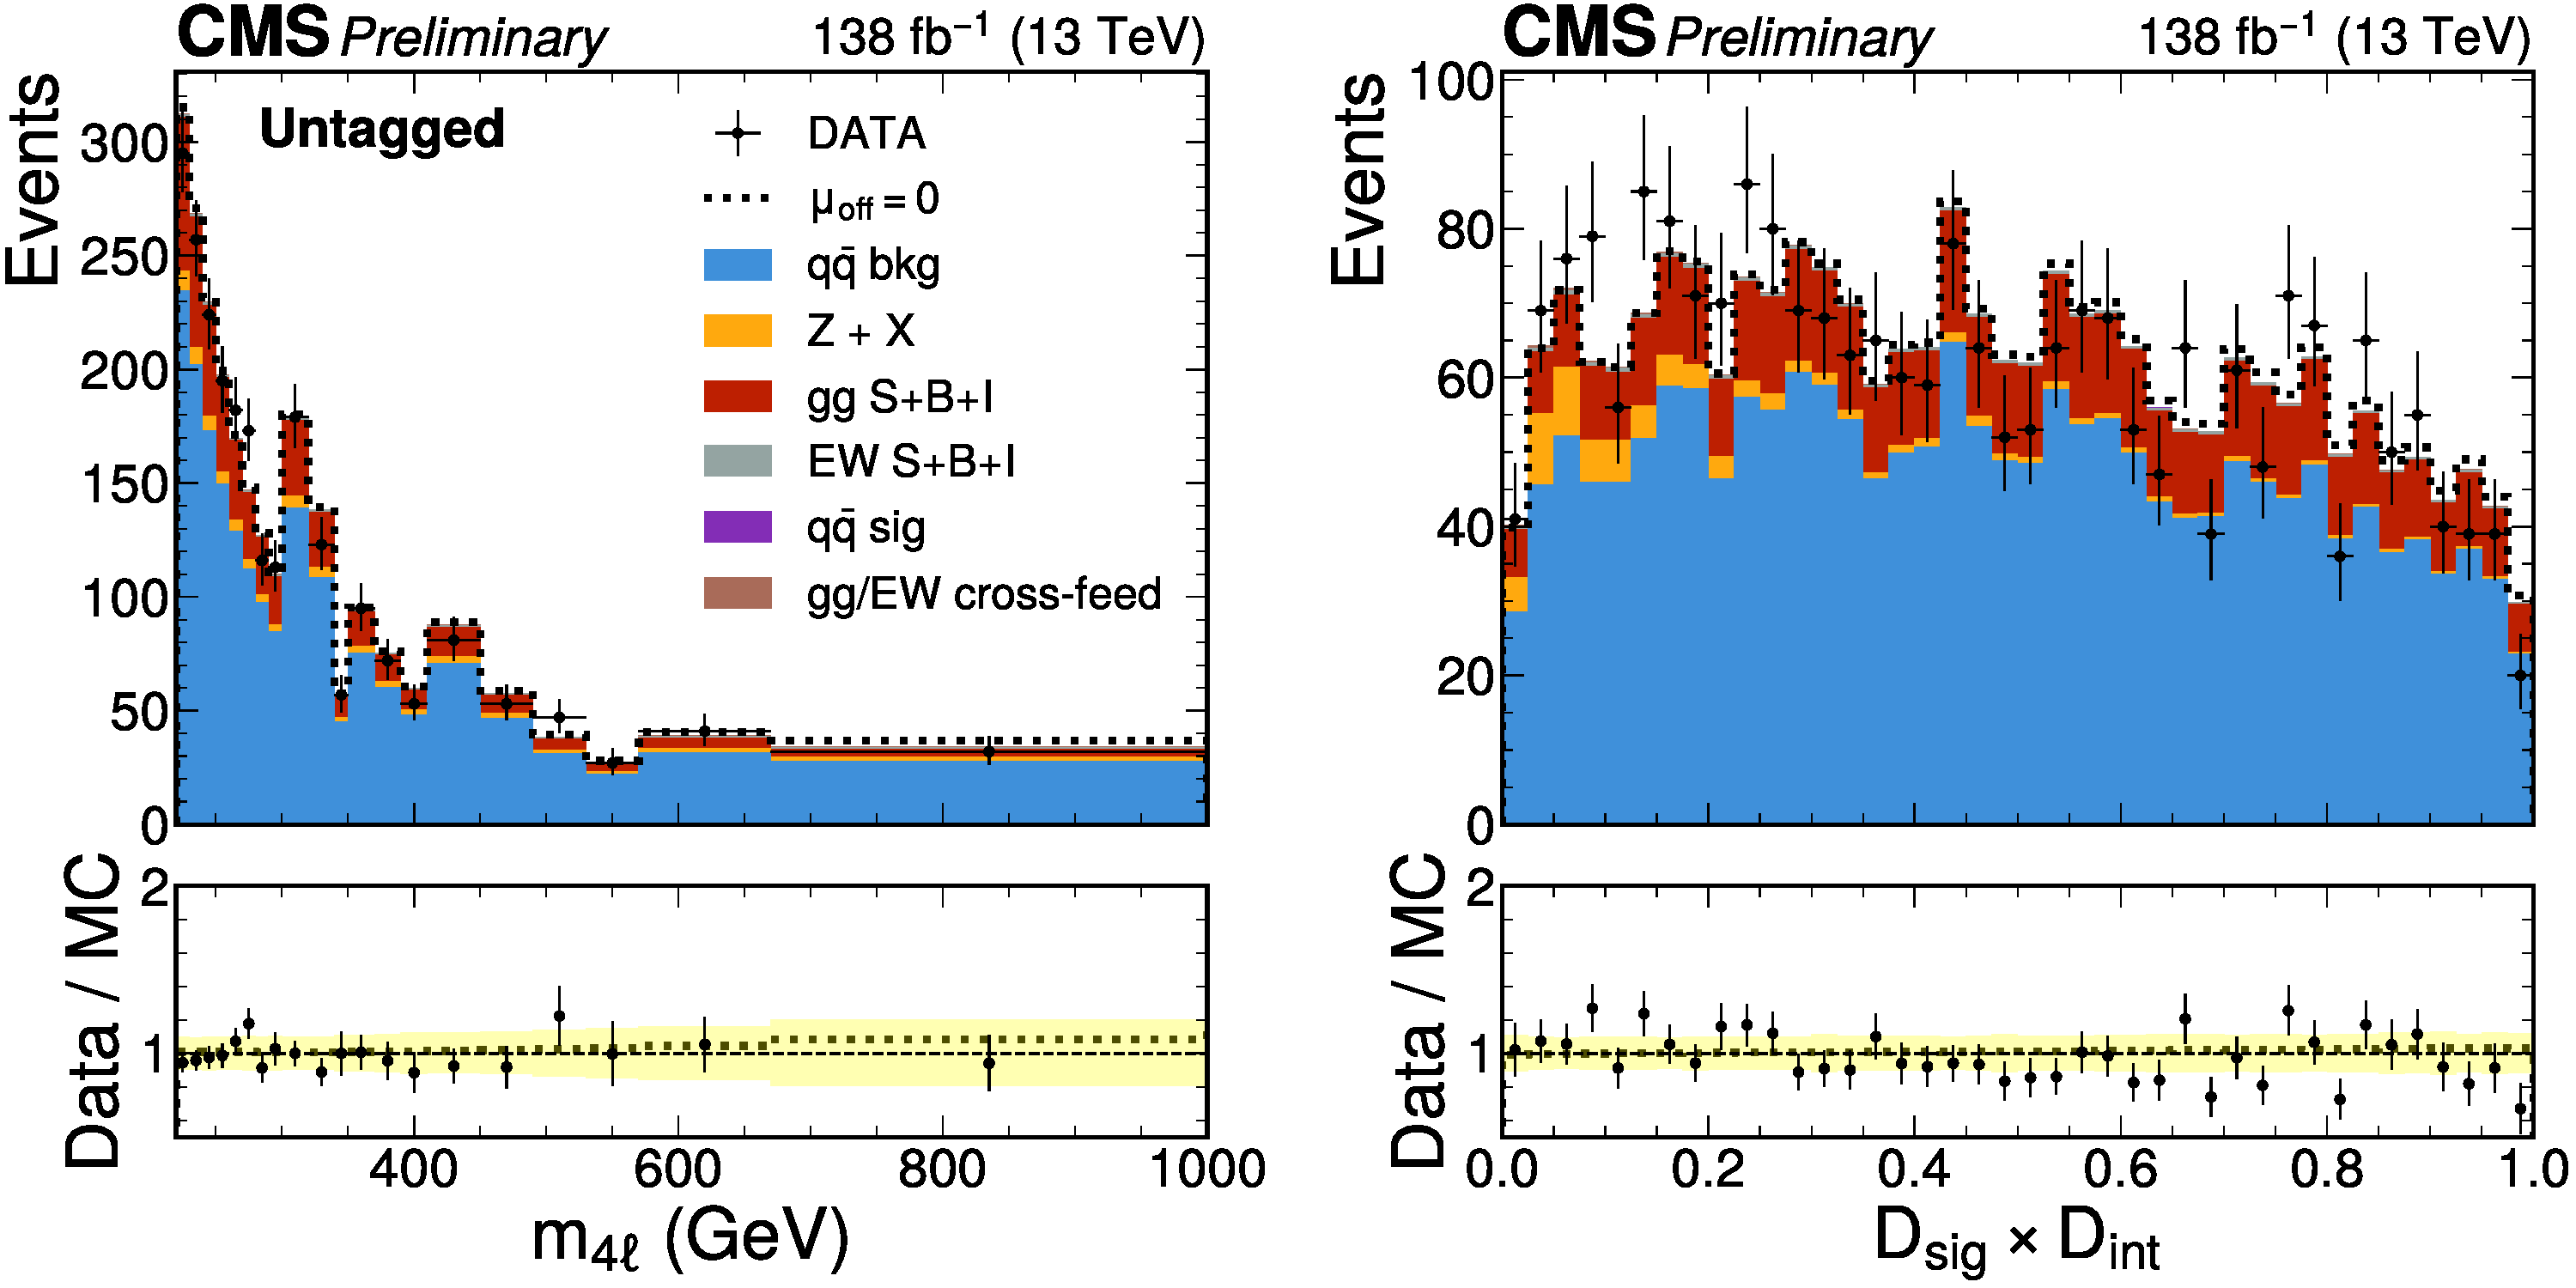
\includegraphics[trim={25.1cm 0 0 0},clip,width=0.55\linewidth]{images/ratio_0.pdf}
\end{center}

\end{block}

\begin{block}{Higgs Substructure}

% Figure~\ref{fig:structure} showcases the evolution given different values of $\Lambda_\text{H}$
% for the form factor described in Eq.~\ref{eq:formFactor}, where $\Lambda_\text{H}$ is the
% energy scale of the form factor and $d$ the characteristic size, 
% which can be with the scan shown in Fig.~\ref{fig:structureScan}.
\begin{align}
  F(q^2) &= 
     \left[
     \frac{1}{1 + | q^2 | / \Lambda_\text{H}^2}
     \right]^2
     \label{eq:formFactor}, &
    d &= \frac{\hbar c}{\Lambda_\text{H}}
\end{align}
% \begin{figure}[!ht]
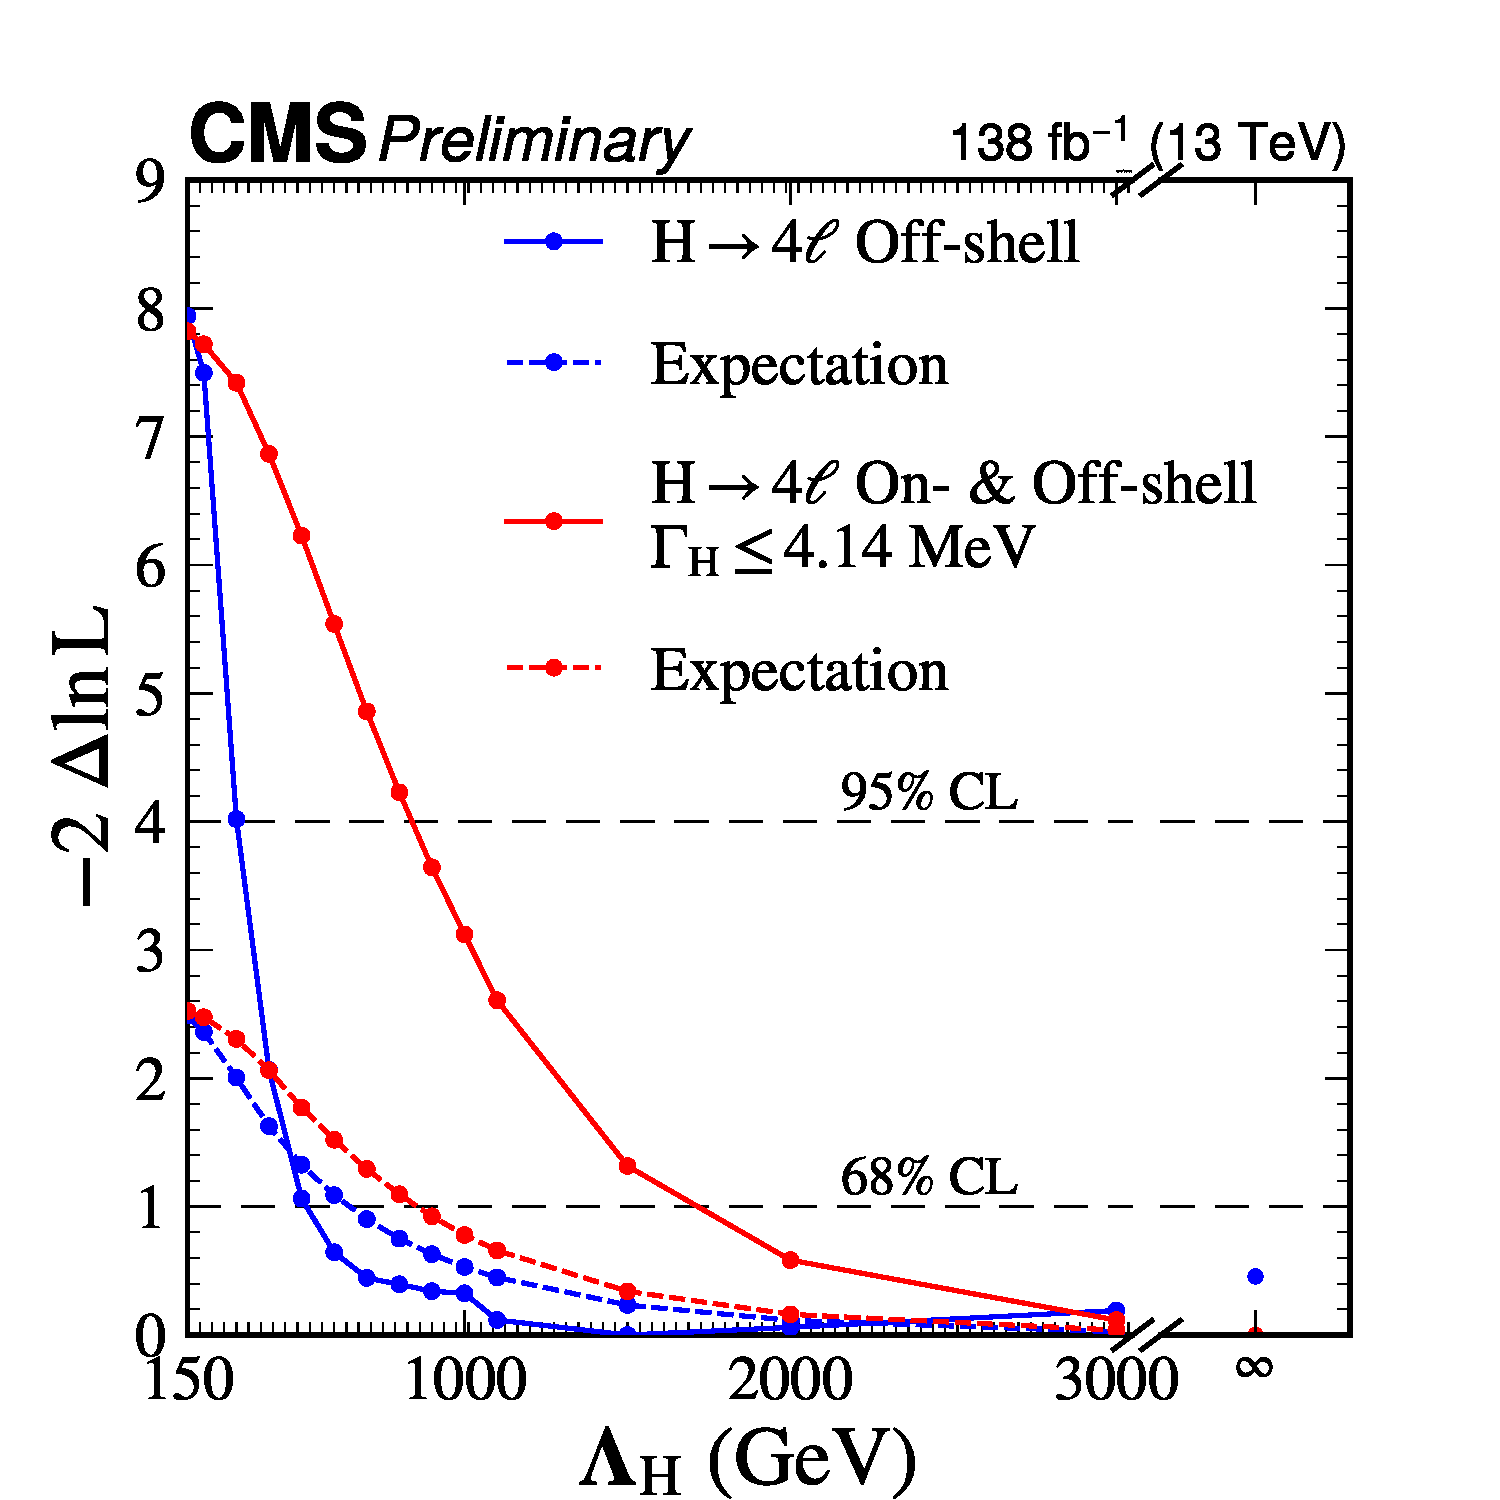
\includegraphics[width=1.05\linewidth]{images/Paper_Structure.pdf}
% \caption{Scan for $\Lambda_\text{H}$}
\label{fig:structureScan}
% \end{figure}
% \begin{table}[!htb]
%   \centering
%   \begin{tabular}{|c | c c | c c |}
%     \hline
%     Scenario & \multicolumn{2}{c |}{Observed (zm)} & \multicolumn{2}{c |}{Expected (zm)} \\
%     & best fit & 95\% CL & best fit & 95\% CL \\
%     \hline
%     off-shell & $130$ & $<660$ & $0$ & ---  \\
%     on+off-shell & $0$ & $<230$ & $0$ & ---  \\
%     \hline
%   \end{tabular}
%   \label{tab:structTab}
% \end{table}
\end{block}

%----------------------------------------------------------------------------------------

%----------------------------------------------------------------------------------------
%	MATHEMATICAL SECTION
%----------------------------------------------------------------------------------------



%----------------------------------------------------------------------------------------

\end{column} % End of column 2.1

\begin{column}{\onecolwid}\vspace{-.6in} % The second column within column 2 (column 2.2)

%----------------------------------------------------------------------------------------
%	METHODS
%----------------------------------------------------------------------------------------

\begin{block}{Yukawa Couplings}
\begin{figure}[!htb]
  \centering
  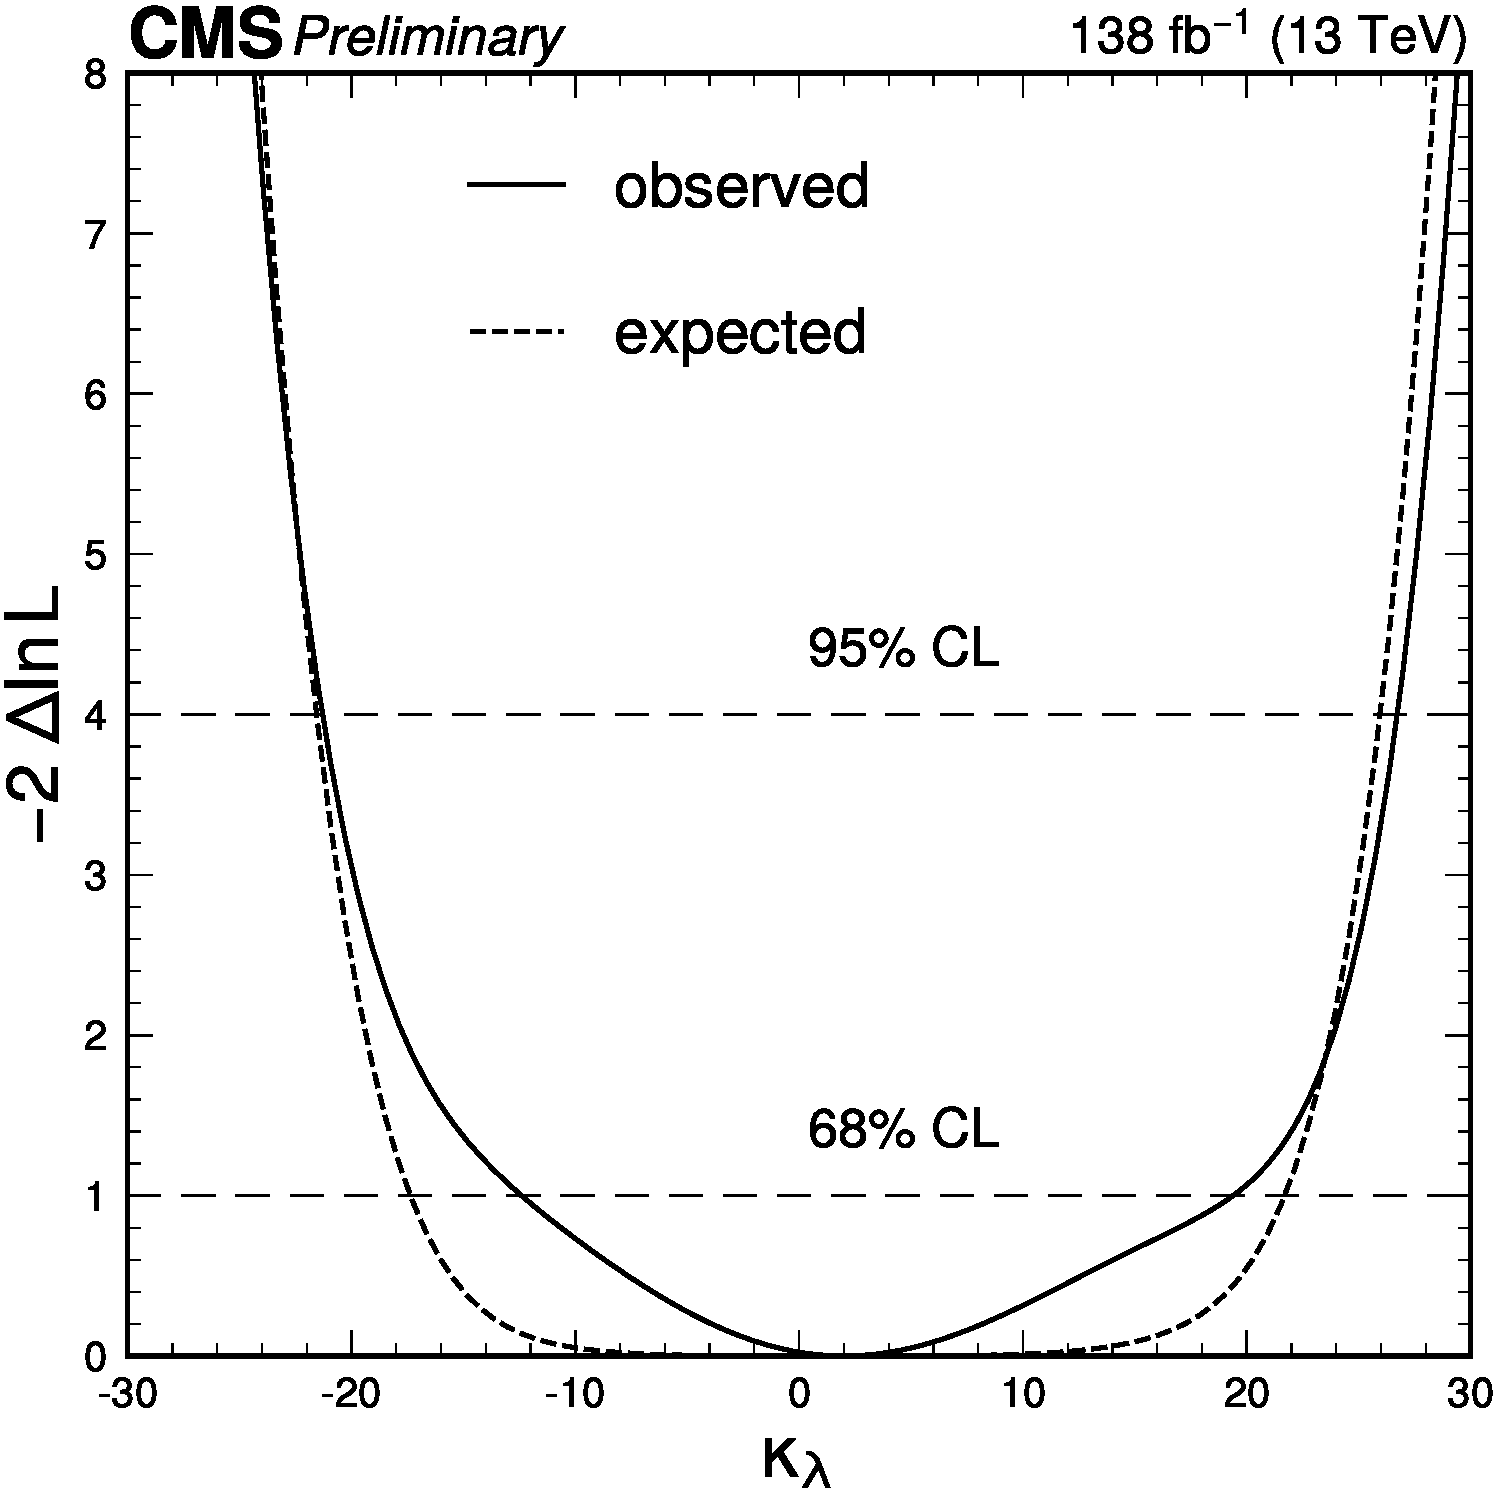
\includegraphics[width=\linewidth]{images/scan_klambda.pdf}
\end{figure}

\end{block}

%----------------------------------------------------------------------------------------

\end{column} % End of column 2.2

\end{columns} % End of the split of column 2 - any content after this will now take up 2 columns width

%----------------------------------------------------------------------------------------
%	IMPORTANT RESULT
%----------------------------------------------------------------------------------------

% \begin{alertblock}{Important Result}

% Lorem ipsum dolor \textbf{sit amet}, consectetur adipiscing elit. Sed commodo molestie porta. Sed ultrices scelerisque sapien ac commodo. Donec ut volutpat elit.

% \end{alertblock} 

%----------------------------------------------------------------------------------------

\begin{columns}[t,totalwidth=\twocolwid] % Split up the two columns wide column again

% \begin{column}{\onecolwid} % The first column within column 2 (column 2.1)



% \end{column} % End of column 2.1

\begin{column}{\onecolwid} % The second column within column 2 (column 2.2)

%----------------------------------------------------------------------------------------
%	RESULTS
%----------------------------------------------------------------------------------------

\begin{block}{Results}

\begin{figure}

\includegraphics[width=0.8\linewidth]{placeholder.jpg}
\caption{Figure caption}
\end{figure}

Nunc tempus venenatis facilisis. Curabitur suscipit consequat eros non porttitor. Sed a massa dolor, id ornare enim:

\begin{table}
\vspace{2ex}
\begin{tabular}{l l l}
\toprule
\textbf{Treatments} & \textbf{Response 1} & \textbf{Response 2}\\
\midrule
Treatment 1 & 0.0003262 & 0.562 \\
Treatment 2 & 0.0015681 & 0.910 \\
Treatment 3 & 0.0009271 & 0.296 \\
\bottomrule
\end{tabular}
\caption{Table caption}
\end{table}

\end{block}

%----------------------------------------------------------------------------------------

\end{column} % End of column 2.2

\end{columns} % End of the split of column 2

\end{column} % End of the second column

\begin{column}{\sepwid}\end{column} % Empty spacer column

\begin{column}{\onecolwid} % The third column

%----------------------------------------------------------------------------------------
%	CONCLUSION
%----------------------------------------------------------------------------------------

\begin{block}{Conclusion}

Nunc tempus venenatis facilisis. \textbf{Curabitur suscipit} consequat eros non porttitor. Sed a massa dolor, id ornare enim. Fusce quis massa dictum tortor \textbf{tincidunt mattis}. Donec quam est, lobortis quis pretium at, laoreet scelerisque lacus. Nam quis odio enim, in molestie libero. Vivamus cursus mi at \textit{nulla elementum sollicitudin}.

\end{block}

%----------------------------------------------------------------------------------------
%	ADDITIONAL INFORMATION
%----------------------------------------------------------------------------------------

\begin{block}{Additional Information}

Maecenas ultricies feugiat velit non mattis. Fusce tempus arcu id ligula varius dictum. 
\begin{itemize}
\item Curabitur pellentesque dignissim
\item Eu facilisis est tempus quis
\item Duis porta consequat lorem
\end{itemize}

\end{block}

%----------------------------------------------------------------------------------------
%	REFERENCES
%----------------------------------------------------------------------------------------

\begin{block}{References}

\nocite{*} % Insert publications even if they are not cited in the poster
\small{\bibliographystyle{unsrt}
\bibliography{sample}\vspace{0.75in}}

\end{block}

%----------------------------------------------------------------------------------------
%	ACKNOWLEDGEMENTS
%----------------------------------------------------------------------------------------

\setbeamercolor{block title}{fg=red,bg=white} % Change the block title color

\begin{block}{Acknowledgements}

\small{\rmfamily{Nam mollis tristique neque eu luctus. Suspendisse rutrum congue nisi sed convallis. Aenean id neque dolor. Pellentesque habitant morbi tristique senectus et netus et malesuada fames ac turpis egestas.}} \\

\end{block}

%----------------------------------------------------------------------------------------
%	CONTACT INFORMATION
%----------------------------------------------------------------------------------------

\setbeamercolor{block alerted title}{fg=black,bg=norange} % Change the alert block title colors
\setbeamercolor{block alerted body}{fg=black,bg=white} % Change the alert block body colors

\begin{alertblock}{Contact Information}

\begin{itemize}
\item Web: \href{http://www.university.edu/smithlab}{http://www.university.edu/smithlab}
\item Email: \href{mailto:john@smith.com}{john@smith.com}
\item Phone: +1 (000) 111 1111
\end{itemize}

\end{alertblock}

\begin{center}
\begin{tabular}{ccc}

\includegraphics[width=0.4\linewidth]{logo.png} & \hfill & 
\includegraphics[width=0.4\linewidth]{logo.png}
\end{tabular}
\end{center}

%----------------------------------------------------------------------------------------

\end{column} % End of the third column

\end{columns} % End of all the columns in the poster

\end{frame} % End of the enclosing frame

\end{document}
